% ============================================================
%  Chapitre 1 — État de l'Art et Analyse de l'Existant
% ============================================================

\chapter{État de l'Art et Analyse de l'Existant}

Ce chapitre positionne Hostifer dans le contexte technologique mondial et algérien. Il présente les modèles de service cloud fondamentaux, analyse les solutions existantes sur le marché international et local, et identifie les lacunes que Hostifer entend combler. Cette analyse constitue la justification technique et économique du projet.

% ============================================================
%  Section 1.1
% ============================================================

\section{Le Cloud Computing et les modèles de service}

Le cloud computing représente l'une des mutations les plus profondes de l'informatique moderne. Le NIST (\textit{National Institute of Standards and Technology}) en donne la définition de référence : le cloud computing est un modèle permettant un accès réseau ubiquitaire, pratique et à la demande à un pool partagé de ressources informatiques configurables (réseaux, serveurs, stockage, applications et services) pouvant être rapidement provisionnées et libérées avec un effort de gestion minimal ou une interaction réduite avec le fournisseur de services.  Ce modèle repose sur cinq caractéristiques essentielles : le libre-service à la demande, l'accès réseau large bande, la mutualisation des ressources, l'élasticité rapide, et la mesure du service \cite{nist-sp800-145}.

Sur la base de cette définition, le NIST distingue trois modèles de service fondamentaux — IaaS, PaaS et SaaS — qui structurent l'ensemble de l'offre cloud commerciale et académique, et qui se différencient par le niveau d'abstraction fourni au consommateur et par la répartition des responsabilités entre le fournisseur et l'utilisateur \cite{nist-sp800-292}.

\subsection*{Infrastructure as a Service (IaaS)}

L'IaaS est une forme de cloud computing qui fournit un accès à la demande à des ressources informatiques hébergées dans le cloud — calcul, stockage et réseau — soit l'infrastructure IT sous-jacente nécessaire à l'exécution des applications et des charges de travail dans le cloud.  Dans ce modèle, le fournisseur cloud gère les couches physiques (matériel, datacenter, virtualisation), tandis que le consommateur conserve le contrôle total sur les systèmes d'exploitation, le stockage, les applications déployées et, partiellement, les composants réseau \cite{nist-sp800-145}. L'IaaS offre la plus grande flexibilité des trois modèles, au prix d'une responsabilité opérationnelle importante : le consommateur doit administrer lui-même les machines virtuelles, les patchs de sécurité, la haute disponibilité et la mise à l'échelle. Des exemples représentatifs de ce modèle incluent Amazon EC2, Google Compute Engine, Microsoft Azure Virtual Machines et Alibaba Cloud ECS.

\subsection*{Platform as a Service (PaaS)}

Le NIST définit le PaaS comme un modèle dans lequel le consommateur déploie sur l'infrastructure cloud des applications qu'il a créées ou acquises, en utilisant les langages de programmation, bibliothèques, services et outils supportés par le fournisseur. Le consommateur ne gère ni ne contrôle l'infrastructure cloud sous-jacente, incluant le réseau, les serveurs, les systèmes d'exploitation ou le stockage, mais dispose d'un contrôle sur les applications déployées et éventuellement sur les paramètres de configuration de l'environnement d'hébergement applicatif. 

Le PaaS constitue ainsi une couche d'abstraction intermédiaire entre l'IaaS et le SaaS : il masque la complexité de l'infrastructure tout en laissant au développeur le contrôle complet de son code applicatif. L'idée fondatrice du PaaS est d'abstraire autant que possible l'infrastructure, afin que les développeurs puissent se concentrer sur la construction et le déploiement de leurs applications, sans gérer les serveurs sous-jacents.  Ce paradigme a été popularisé par Heroku, la première plateforme à avoir rendu le déploiement d'applications web accessible sans compétences en administration système, introduisant ainsi le concept de PaaS à la communauté des développeurs au sens large. Une nouvelle génération de plateformes PaaS — Vercel, Railway, Render, Fly.io — a depuis émergé, offrant une expérience développeur améliorée, une tarification plus transparente et un support natif des conteneurs \cite{paas-comparison}.

\subsection*{Software as a Service (SaaS)}

Le NIST définit le SaaS comme un modèle de service dans lequel le consommateur ne gère ni ne contrôle l'infrastructure cloud sous-jacente, incluant le réseau, les serveurs, les systèmes d'exploitation, le stockage, ni même les capacités individuelles de l'application, à l'exception possible de paramètres de configuration applicatifs limités propres à l'utilisateur.  Le SaaS représente le niveau d'abstraction maximal : l'utilisateur consomme une application complète livrée via un navigateur web ou une API, sans aucune responsabilité technique sur la pile logicielle ou l'infrastructure. Des exemples emblématiques incluent Google Workspace, Microsoft 365, Salesforce, et Notion.

\subsection*{Le modèle de responsabilité partagée}

La distinction fondamentale entre ces trois modèles réside dans la répartition des responsabilités entre le fournisseur et le consommateur. La Figure~\ref{fig:cloud-models} illustre cette pyramide de responsabilités : plus on monte vers le SaaS, plus le fournisseur prend en charge de couches, et moins le consommateur a de contrôle mais aussi de charge opérationnelle. Le Tableau~\ref{tab:shared-responsibility} détaille cette répartition couche par couche pour les trois modèles.

Le SaaS offre un confort maximal avec une gestion minimale, le PaaS apporte une flexibilité de développement, et l'IaaS fournit un contrôle de l'infrastructure avec une responsabilité opérationnelle complète. De nombreuses organisations utilisent simultanément plusieurs modèles de service pour optimiser différentes fonctions métiers. 

\subsection*{Positionnement de Hostifer dans le modèle PaaS}

Hostifer se positionne clairement dans la catégorie \textbf{PaaS}, en adoptant les principes fondamentaux de ce modèle tout en les instanciant sur une infrastructure Kubernetes native. Comme les plateformes PaaS de référence, Hostifer abstrait intégralement la gestion de l'infrastructure sous-jacente — provisionnement des conteneurs, configuration réseau, émission des certificats TLS, gestion des secrets — et n'expose à l'utilisateur qu'une interface simple orientée vers le code source : fournir une URL de dépôt GitHub suffit pour déclencher le déploiement complet d'une application. Le développeur conserve le contrôle total de son code applicatif, de ses variables d'environnement et de la configuration de son pipeline CI/CD, sans jamais interagir directement avec les primitives Kubernetes.

Ce positionnement PaaS se distingue cependant des offres internationales existantes sur deux axes déterminants. D'une part, Hostifer repose sur une infrastructure Kubernetes \textit{multi-tenant native}, où chaque application est isolée dans son propre namespace Kubernetes avec des politiques réseau, des quotas de ressources et une gestion des secrets dédiés — une granularité d'isolation que les PaaS traditionnels basés sur des conteneurs partagés ne proposent pas systématiquement. D'autre part, Hostifer est conçu pour et hébergé en Algérie, avec une tarification en dinars algériens (DZD) et une conformité aux lois 18-07 et 25-11 sur la protection des données personnelles — des caractéristiques structurellement impossibles à offrir pour les plateformes étrangères et absentes des initiatives locales existantes, comme analysé dans les sections suivantes.
\begin{figure}[h]
    \centering
    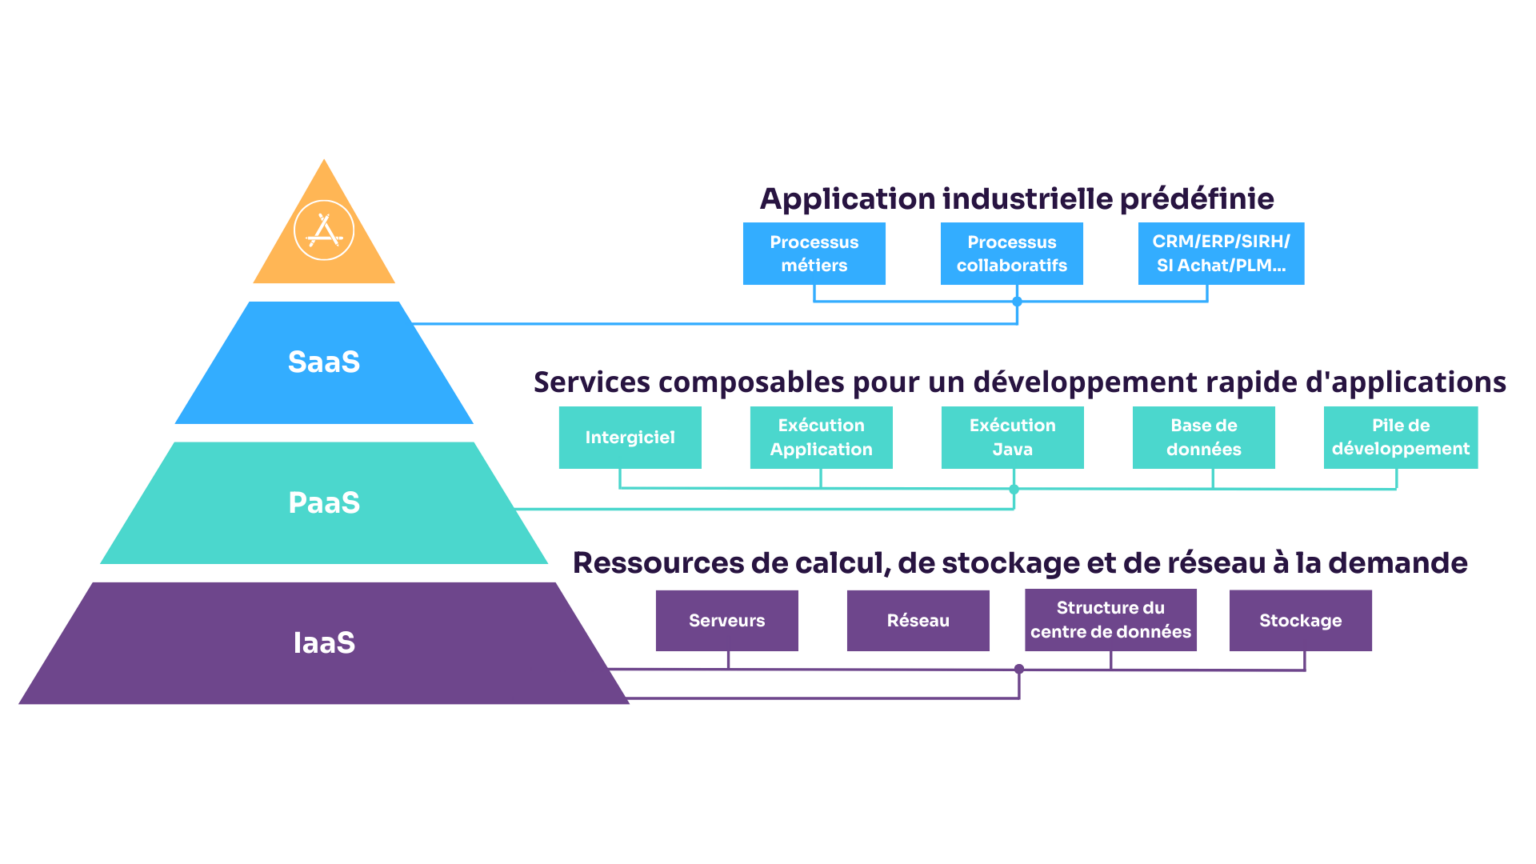
\includegraphics[width=1\linewidth]{5-Chapters/Chapter1/figures/modeles-cloud.png}
    \caption{Pyramide des modèles de service cloud (IaaS / PaaS / SaaS) avec exemples de plateformes pour chaque niveau}
    \label{fig:1.1}
\end{figure}

\begin{table}[h]
    \centering
    \caption{Comparaison des responsabilités client/fournisseur dans les trois modèles}
    \label{tab:1.1}
	\label{tab:shared-responsibility}
    \begin{tabular}{p{3.5cm} p{3.8cm} p{3.8cm} p{3.8cm}}
        \hline
        \textbf{Critère} & \textbf{IaaS} & \textbf{PaaS} & \textbf{SaaS} \\
        \hline
        Infrastructure physique & Fournisseur & Fournisseur & Fournisseur \\
        \hline
        Système d'exploitation & Client & Fournisseur & Fournisseur \\
        \hline
        Plateforme d'exécution / middleware & Client & Fournisseur & Fournisseur \\
        \hline
        Application & Client & Client & Fournisseur \\
        \hline
        Données et configuration métier & Client & Client & Client / partiellement fournisseur selon le service \\
        \hline
    \end{tabular}
\end{table}

% ============================================================
%  Section 1.2
% ============================================================

\section{L'orchestration de conteneurs — Docker et Kubernetes}

\subsection{La conteneurisation avec Docker et l'OCI}

La conteneurisation est une technologie de virtualisation légère qui permet d'encapsuler une application et l'ensemble de ses dépendances — bibliothèques, fichiers de configuration, variables d'environnement — dans une unité portable et autonome appelée conteneur. Contrairement à la virtualisation traditionnelle basée sur des machines virtuelles, un conteneur partage le noyau du système d'exploitation hôte et n'embarque que les couches logicielles strictement nécessaires à l'application. Cette architecture réduit considérablement l'empreinte mémoire, accélère le démarrage des instances et garantit la reproductibilité de l'environnement d'exécution entre les phases de développement, de test et de production \cite{docker-docs}.

Docker, lancé en 2013 par la société dotCloud (rebaptisée Docker Inc.), a popularisé la conteneurisation auprès de la communauté des développeurs en proposant un outillage accessible pour la construction, la distribution et l'exécution de conteneurs. Son succès a conduit à la création, en juin 2015, de l'\textit{Open Container Initiative} (OCI) sous l'égide de la Linux Foundation. L'OCI a été lancée par Docker, CoreOS et d'autres acteurs de l'industrie des conteneurs dans le but de créer des standards ouverts pour les formats de conteneurs et les runtimes. Elle comprend aujourd'hui trois spécifications : la spécification de runtime (\textit{runtime-spec}), la spécification d'image (\textit{image-spec}) et la spécification de distribution (\textit{distribution-spec}).  Ces standards garantissent l'interopérabilité entre les outils de l'écosystème : une image construite avec Docker peut être exécutée par containerd, Podman ou tout autre runtime conforme OCI, et stockée dans n'importe quel registre OCI-compatible.

Une image OCI est structurée en couches superposées (\textit{layers}) immuables, chaque couche représentant un ensemble de modifications du système de fichiers par rapport à la couche précédente. Ce mécanisme permet la réutilisation et la mise en cache des couches communes entre différentes images, réduisant les temps de téléchargement et l'espace de stockage consommé. Dans le contexte de Hostifer, le daemon Buildkitd exploite précisément cette structure en couches pour optimiser les builds répétés d'une même application via un cache de couches persistant \cite{buildkit-client}.

\subsection{Kubernetes comme standard d'orchestration}

La conteneurisation seule ne résout pas les problèmes opérationnels liés au déploiement à grande échelle : comment assurer la haute disponibilité, la mise à l'échelle automatique, le rééquilibrage de charge, la gestion des pannes et la mise à jour sans interruption d'un ensemble de conteneurs distribués sur une flotte de machines ? Ces problématiques sont adressées par les orchestrateurs de conteneurs, dont Kubernetes (\texttt{k8s}) s'est imposé comme le standard industriel de référence \cite{k8s-concepts}.

Kubernetes est un projet open source initialement développé par Google, publié en 2014 et confié à la Cloud Native Computing Foundation (CNCF) en 2016. Il automatise le déploiement, la mise à l'échelle et la gestion des applications conteneurisées sur un cluster de machines. Son architecture repose sur un plan de contrôle (\textit{control plane}) composé de l'\texttt{API Server}, du \texttt{Scheduler}, du \texttt{Controller Manager} et d'\texttt{etcd} (le magasin de données distribué de l'état du cluster), et d'un plan de données (\textit{data plane}) constitué des nœuds de travail (\textit{worker nodes}) exécutant les conteneurs applicatifs via un \textit{kubelet} et un runtime conforme CRI (\textit{Container Runtime Interface}). La Figure~\ref{fig:k8s-architecture} illustre cette architecture.

\subsection{Concepts clés de Kubernetes}

La compréhension de l'implémentation de Hostifer nécessite la maîtrise de sept ressources Kubernetes fondamentales, décrites ci-après.

\textbf{Pod.} Le Pod est l'unité d'exécution atomique de Kubernetes. Il encapsule un ou plusieurs conteneurs partageant le même espace réseau (adresse IP unique, ports) et le même espace de stockage (\textit{volumes}). Kubernetes garantit que les conteneurs au sein d'un Pod partagent le même namespace réseau et peuvent communiquer entre eux via \texttt{localhost}.  Dans la grande majorité des cas, un Pod contient un seul conteneur applicatif. Les Pods sont éphémères : s'ils tombent en panne, Kubernetes les recrée automatiquement, potentiellement sur un nœud différent, d'où l'importance des ressources d'abstraction supérieures telles que les Deployments et les Services.

\textbf{Namespace.} Un Namespace est une partition logique du cluster Kubernetes, permettant d'isoler des groupes de ressources au sein d'un même cluster physique. Les Namespaces constituent un excellent moyen de séparer des environnements (développement, staging, production) ou d'isoler les workloads de différentes équipes.  Ils servent de périmètre d'application pour les politiques de sécurité réseau, les quotas de ressources et les règles RBAC. Dans Hostifer, chaque application déployée par un utilisateur est provisionnée dans un Namespace Kubernetes dédié, réalisant ainsi le modèle d'isolation silo décrit dans la section 2.5.2 \cite{k8s-concepts}.

\textbf{Deployment.} Un Deployment est un contrôleur Kubernetes qui gère le cycle de vie d'un ensemble de Pods identiques (\textit{ReplicaSet}). Il garantit qu'un nombre spécifié de réplicas du Pod est en cours d'exécution à tout moment, gère les mises à jour progressives (\textit{rolling updates}) sans interruption de service, et assure le retour arrière vers une version précédente en cas d'échec. Le Deployment est la ressource de déploiement standard pour les applications stateless dans Kubernetes.

\textbf{Service.} Un Service est une abstraction réseau qui expose un ensemble de Pods sous une adresse IP virtuelle stable et un nom DNS fixe, indépendamment des adresses IP éphémères des Pods individuels. Les Pods étant dynamiques et leurs adresses IP pouvant être réassignées lors des mises à l'échelle ou des redémarrages, un Service agit comme un endpoint stable qui abstrait les IPs des Pods et offre un équilibrage de charge, une découverte de service et une abstraction réseau.  Kubernetes propose plusieurs types de Services : \texttt{ClusterIP} (accessible uniquement en interne au cluster), \texttt{NodePort} (exposé sur un port de chaque nœud), et \texttt{LoadBalancer} (intégrant un équilibreur de charge cloud externe).

\textbf{Ingress.} L'Ingress est une ressource Kubernetes qui gère l'accès HTTP et HTTPS depuis l'extérieur du cluster vers les Services internes. L'Ingress permet de définir des règles de routage basées sur l'URL pour distribuer les routes HTTP/HTTPS vers différents Services backend ; les requêtes sont ensuite transmises aux Pods correspondants de chaque Service.  L'Ingress nécessite un contrôleur d'entrée (\textit{Ingress Controller}) déployé dans le cluster pour implémenter ces règles ; Hostifer utilise Traefik comme contrôleur d'entrée, qui expose des ressources CRD étendues telles que l'\texttt{IngressRoute} décrite dans la section 3.4.1.

\textbf{ResourceQuota.} Un ResourceQuota définit des contraintes agrégées sur les ressources consommables dans un Namespace. Les ResourceQuotas plafonnent la consommation totale de ressources d'un namespace en définissant des limites dures sur les \texttt{requests.cpu}, \texttt{requests.memory}, les \texttt{limits.cpu} et \texttt{limits.memory}, ainsi que sur le nombre total d'objets Kubernetes de différents types.  Lorsqu'un utilisateur tente de créer une ressource qui dépasse le quota défini, la création est rejetée par l'API server. Dans Hostifer, les ResourceQuotas sont utilisés pour garantir que chaque tenant ne peut consommer que les ressources correspondant à son plan tarifaire souscrit, préservant l'isolation et l'équité entre tenants.

\textbf{NetworkPolicy.} Une NetworkPolicy est une ressource Kubernetes qui définit les règles de contrôle du trafic réseau entre les Pods ou entre les Pods et des endpoints externes. Une NetworkPolicy agit comme un pare-feu, appliquant des règles d'entrée (ingress) et de sortie (egress) pour sécuriser le trafic dans le cluster.  Par défaut, sans aucune NetworkPolicy appliquée, tous les Pods d'un cluster Kubernetes peuvent communiquer librement entre eux. L'application d'une NetworkPolicy de type \textit{default-deny} transforme ce modèle permissif en un modèle \textit{allowlist} strict, où seul le trafic explicitement autorisé peut transiter. Il convient de noter qu'une NetworkPolicy n'a d'effet que si un plugin réseau capable d'appliquer ces politiques est installé dans le cluster — parmi les plus courants : Calico, Cilium, Kube-router et Weave Net.  L'implémentation Hostifer s'appuie sur ce mécanisme pour garantir l'isolation réseau inter-tenant décrite dans la section 2.5.2.

Le cycle de vie d'un Pod Kubernetes, depuis son état \texttt{Pending} jusqu'aux états terminaux \texttt{Succeeded} ou \texttt{Failed}, est illustré dans la Figure~\ref{fig:pod-lifecycle}.

\begin{figure}[h]
	\centering
	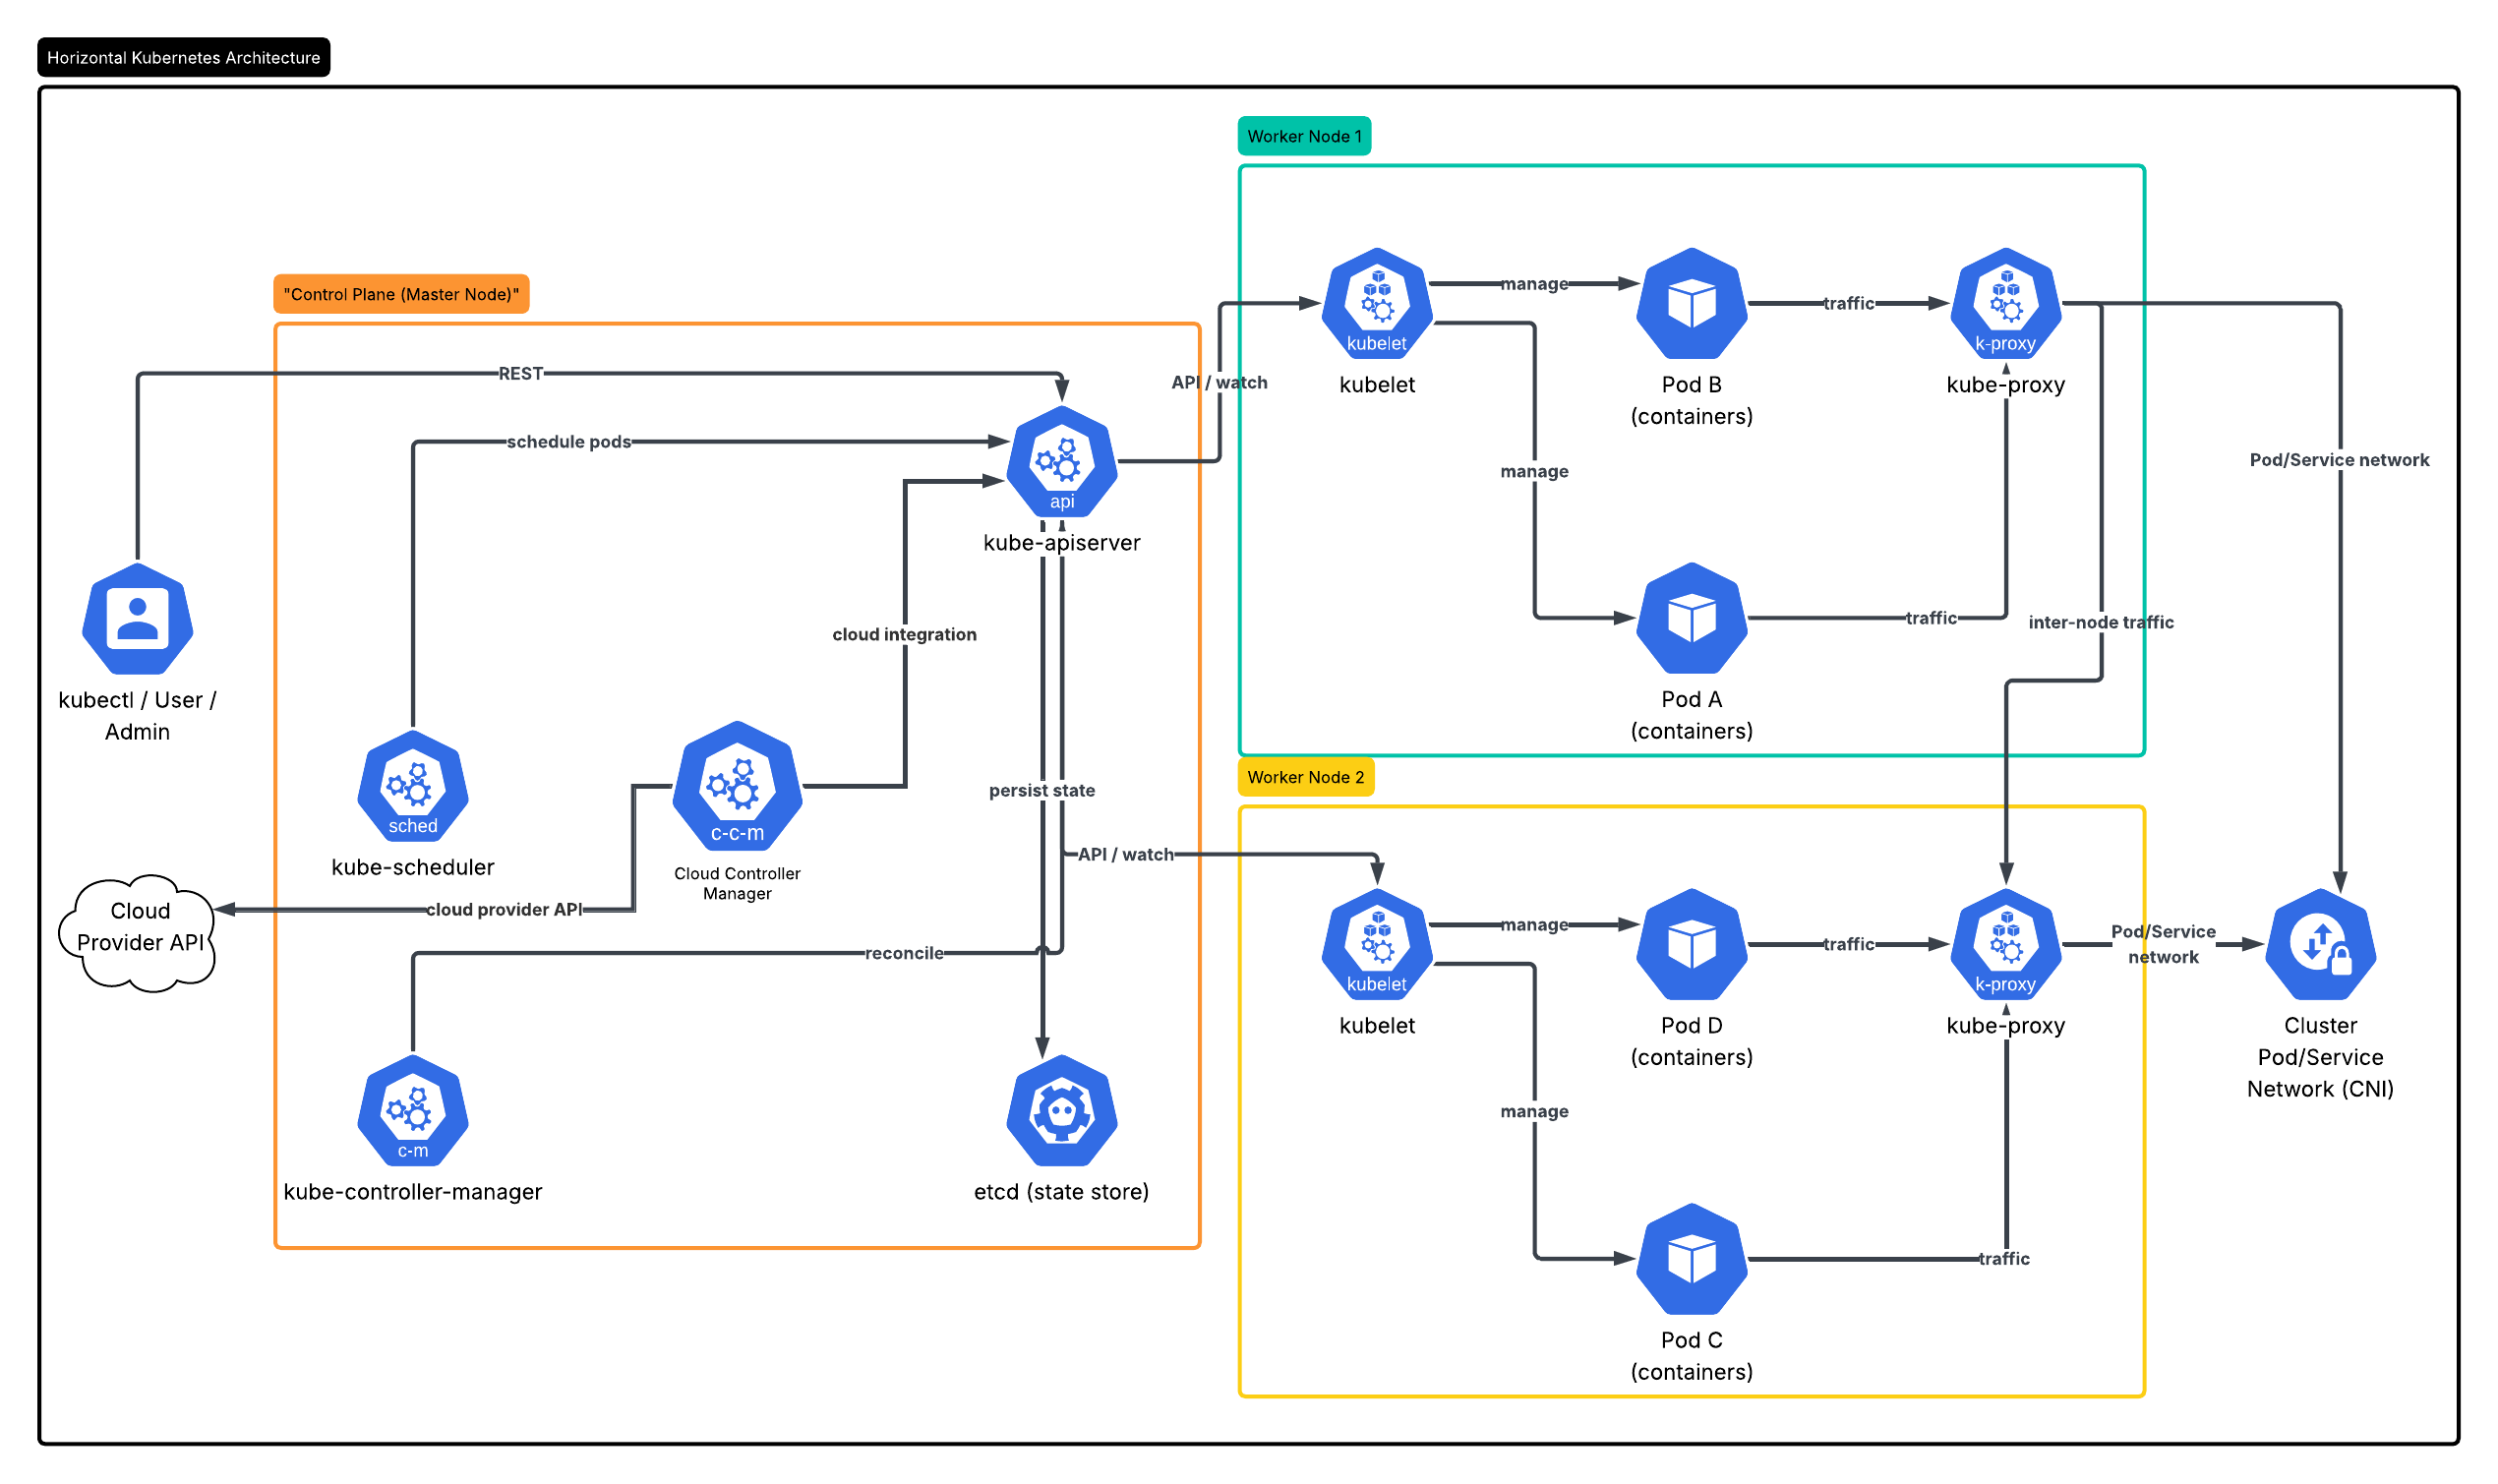
\includegraphics[width=1\linewidth]{5-Chapters/Chapter1/figures/Kubernetes_Architecture.png}
	\caption{Architecture d'un cluster Kubernetes (Master node, Worker nodes, etcd, API Server)}
	\label{fig:1.2}
	\label{fig:pod-lifecycle}
\end{figure}

\begin{figure}[h]
	\centering
	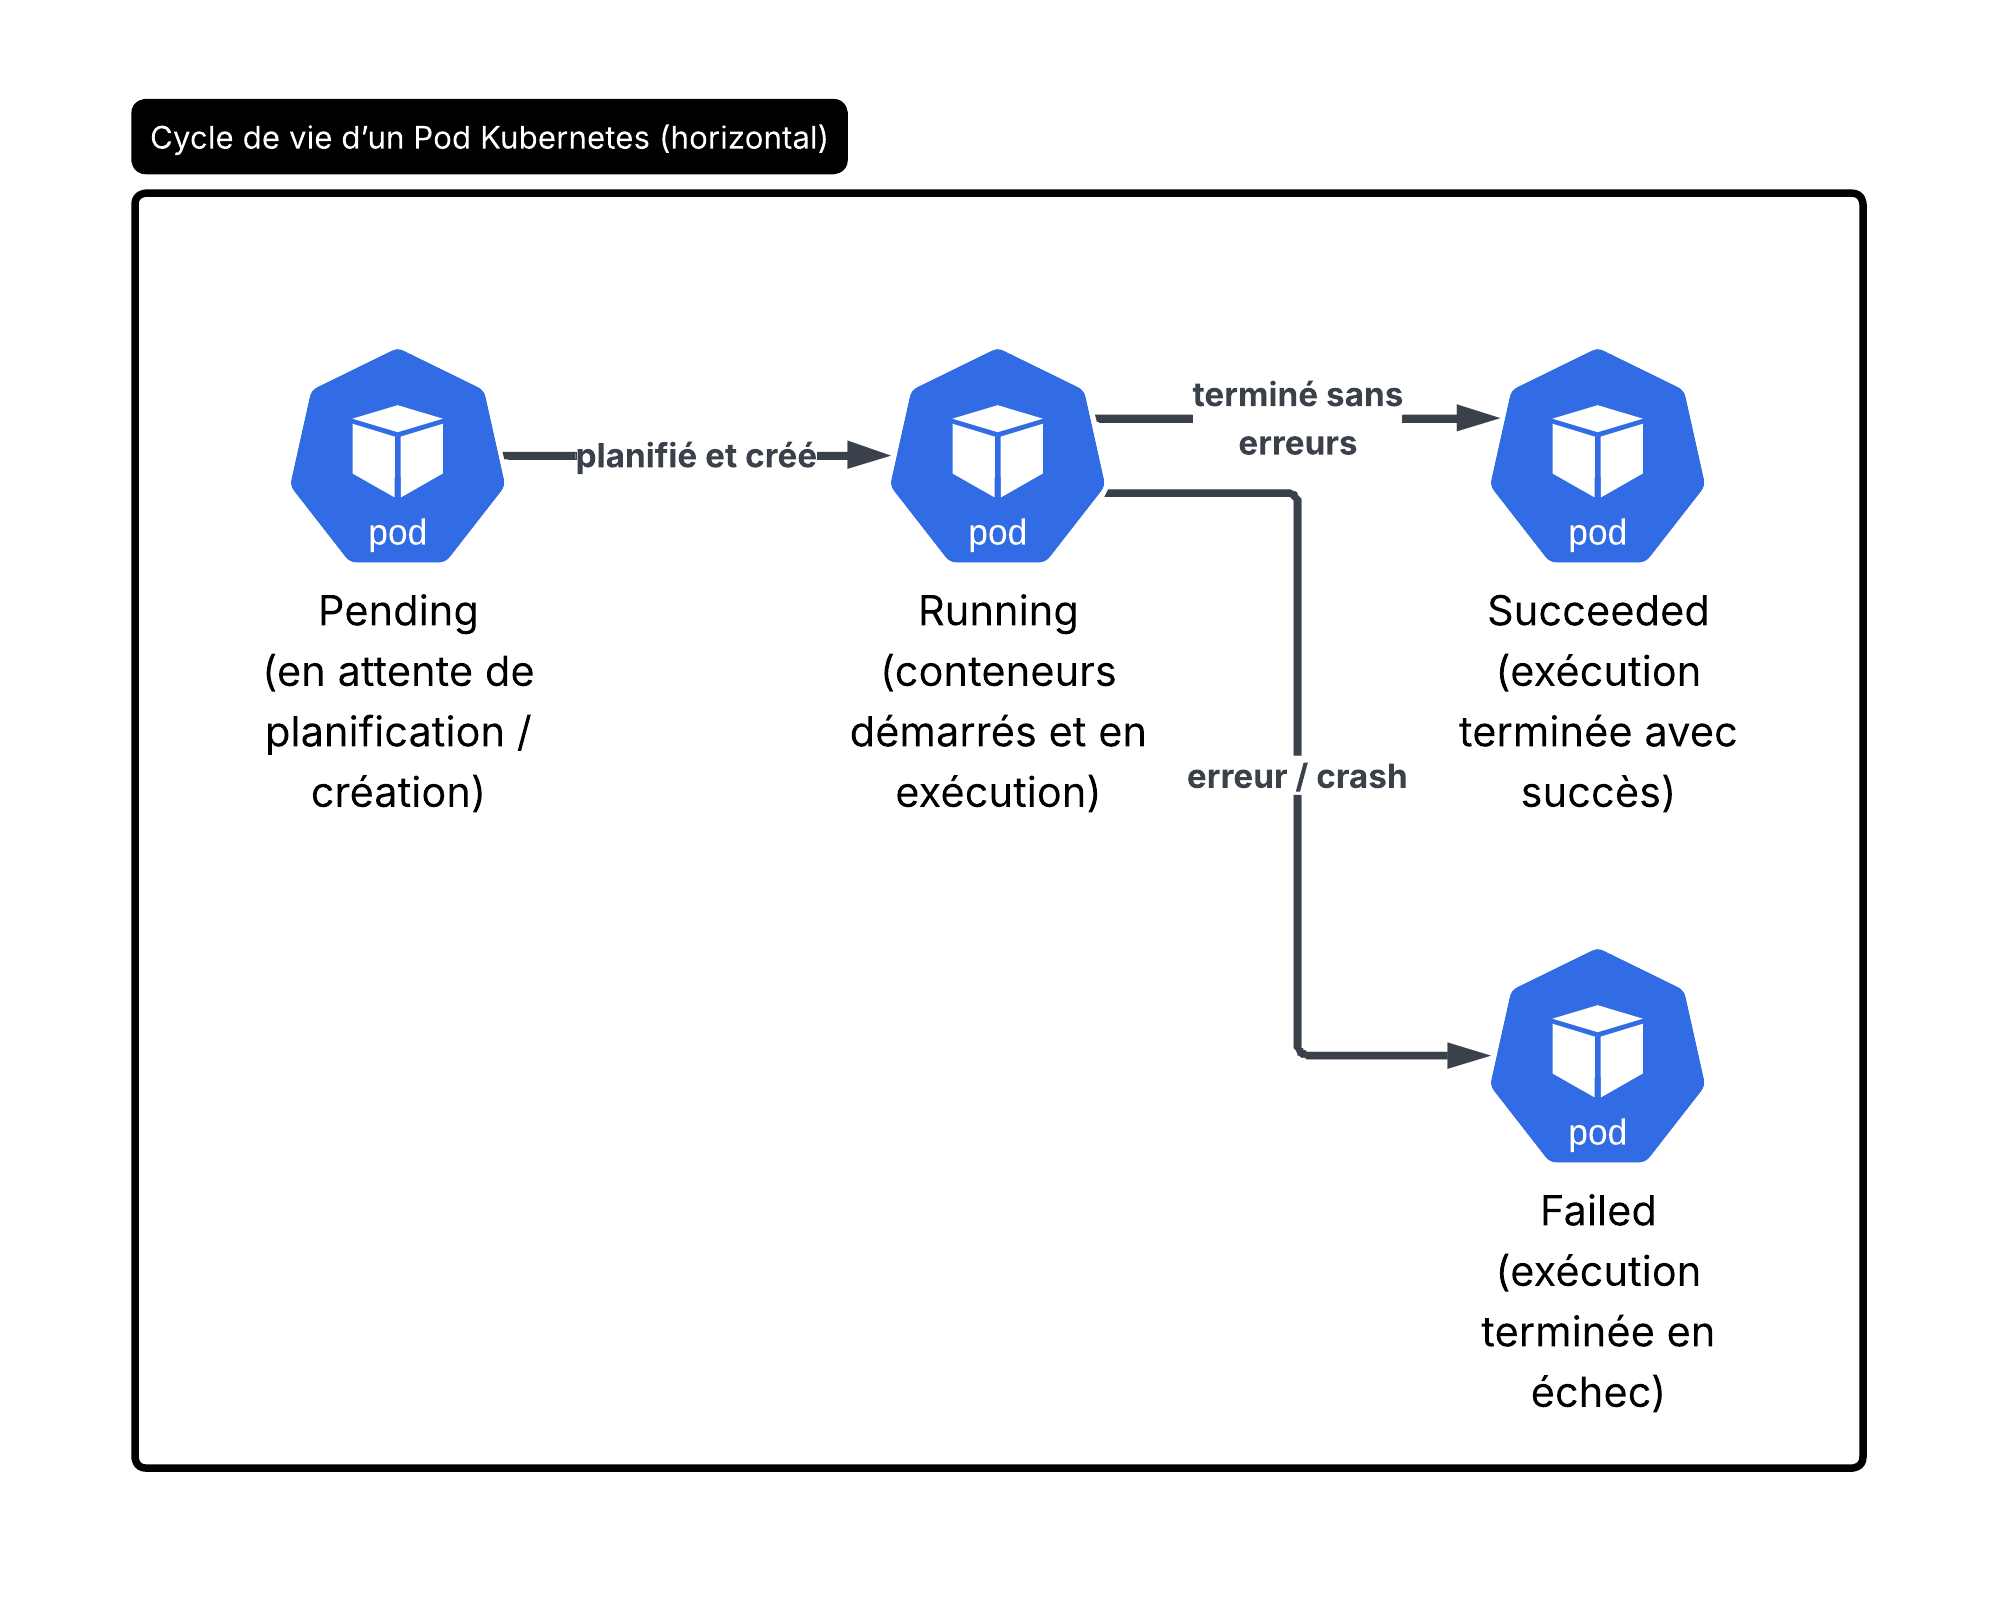
\includegraphics[width=1\linewidth]{5-Chapters/Chapter1/figures/pod_lifecycle.png}
	\caption{Cycle de vie d'un Pod Kubernetes (Pending → Running → Succeeded/Failed)}
	\label{fig:1.3}
\end{figure}

% ============================================================
%  Section 1.3
% ============================================================

\section{Analyse des plateformes PaaS internationales}

Le marché des plateformes PaaS pour développeurs a connu une croissance significative depuis 2010, portée d'abord par Heroku qui a défini le paradigme du déploiement depuis un dépôt Git, puis par une nouvelle génération de plateformes nées de la fin du tier gratuit Heroku en 2022. Cette section analyse les six plateformes les plus représentatives du marché international, en évaluant pour chacune son modèle de déploiement, ses technologies sous-jacentes, sa tarification et ses limitations structurelles pour le contexte algérien \cite{paas-comparison}.

\subsection*{Vercel}

Vercel est une plateforme PaaS fondée en 2015, initialement sous le nom ZEIT, et créatrice du framework Next.js. Vercel se concentre sur les développeurs frontend et l'architecture Jamstack. Elle excelle dans le déploiement de sites statiques et de fonctions serverless, et offre une excellente expérience développeur avec une interface de déploiement soignée.  Son modèle de déploiement est hybride : les assets statiques sont distribués directement sur un CDN mondial, tandis que les fonctions backend sont exécutées en tant que fonctions serverless dans des conteneurs légers de type Lambda sur l'infrastructure AWS sous-jacente.

La force de Vercel réside dans son intégration native avec Next.js et son réseau edge mondial qui garantit des temps de réponse très faibles pour les applications frontend. Cependant, Vercel n'est pas adapté aux charges de travail longue durée, incluant le traitement de données ETL, le transcodage média, la génération de rapports, les tâches DevOps/infrastructure, ou toute charge nécessitant une connexion persistante.  Sa tarification, exprimée en USD avec un plan pro à 20~\$/mois, est inaccessible via les moyens de paiement algériens standards, et ses serveurs sont localisés exclusivement aux États-Unis, en Europe et en Asie, ce qui exclut toute conformité à la loi 18-07 sur la localisation des données personnelles des ressortissants algériens.

\subsection*{Railway}

Railway est une plateforme PaaS lancée en 2020 qui cible les développeurs souhaitant déployer rapidement des applications backend complètes, incluant des bases de données. Railway est la meilleure alternative à Heroku pour les applications de petite et moyenne taille. Elle propose une configuration plus facile, une meilleure tarification et une expérience développeur plus moderne. Railway supporte le déploiement depuis un Dockerfile ou via la détection automatique de stack via Nixpacks ou Railpacks. 

Sur le plan technique, Railway est précisément l'un des créateurs de Railpack — l'outil de détection de framework et de génération de plans de build utilisé dans Hostifer — ce qui témoigne de son investissement dans l'outillage de build automatisé. Railway propose une configuration en un clic pour PostgreSQL, MySQL, Redis et MongoDB, et permet de déployer toute base de données fonctionnant dans un conteneur Docker.  Sa tarification est basée sur la consommation (\textit{usage-based}), avec une facturation à la seconde d'utilisation des ressources. Comme pour l'ensemble des plateformes internationales analysées, la tarification est exclusivement en USD, les régions de déploiement disponibles sont limitées à l'Amérique du Nord, l'Europe et l'Asie, et aucun mécanisme de conformité réglementaire algérien n'est prévu ou envisageable dans leur modèle économique.

\subsection*{Render}

Render est une plateforme PaaS lancée en 2019 qui se positionne comme une alternative à Heroku avec une tarification mensuelle prévisible par instance. Render propose un ensemble de fonctionnalités similaire à Heroku avec quelques améliorations, mais maintient une tarification traditionnelle basée sur les instances, ce qui la rend plus prévisible que les modèles usage-based de Railway ou Fly.io.  Elle supporte le déploiement d'applications web, de workers en arrière-plan, de tâches cron et de bases de données PostgreSQL managées.

Render se distingue par son support natif du déploiement multi-région et par une interface utilisateur claire orientée vers les développeurs débutants. Elle offre également une gestion des \textit{Infrastructure as Code} via des fichiers \texttt{render.yaml} (\textit{blueprints}), permettant de versionner la configuration d'infrastructure dans le dépôt Git. Ses limitations pour le contexte algérien sont identiques aux autres plateformes internationales : facturation en USD, absence de région Afrique du Nord, et aucune conformité possible avec les obligations de résidence des données imposées par la loi 25-11.

\subsection*{Heroku}

Heroku, acquis par Salesforce en 2010, est la plateforme qui a fondé et popularisé le paradigme PaaS tel qu'il est connu aujourd'hui. Heroku est une plateforme PaaS mature qui abstrait la complexité de l'infrastructure, permettant aux développeurs de se concentrer sur le code applicatif. Elle supporte plusieurs langages de programmation et fournit un écosystème robuste d'add-ons pour étendre les applications.  Son modèle de déploiement repose sur le concept de \textit{dynos} — des conteneurs légers exécutant les processus déclarés dans un fichier \texttt{Procfile}.

La fin du tier gratuit Heroku en novembre 2022 a provoqué une migration massive de ses utilisateurs vers Railway, Render et Fly.io. Sa tarification, significativement plus élevée que ses concurrents modernes pour des fonctionnalités équivalentes, combinée à une dette technologique accumulée depuis plus d'une décennie, a considérablement érodé sa position sur le marché des développeurs indépendants. Pour le contexte algérien, Heroku cumule toutes les limitations des plateformes internationales : tarification USD, infrastructure hébergée sur AWS (régions US/EU/AP), et absence totale de mécanismes de conformité réglementaire locale.

\subsection*{Fly.io}

Fly.io adopte une approche architecturale distinctive parmi les plateformes PaaS : plutôt que d'exécuter les applications dans des conteneurs Docker traditionnels, elle s'appuie sur Firecracker, la technologie de microVM développée par AWS. Fly.io déploie les applications conteneurisées sous forme de Firecracker microVMs dans plus de 18 régions mondiales, exécutant le calcul au plus près des utilisateurs pour réduire la latence. Chaque application bénéficie d'un réseau maillé WireGuard privé par défaut, permettant une communication sécurisée inter-services entre régions sans configuration. 

Firecracker est une technologie de microVMs légères qui combine les propriétés de sécurité et d'isolation des VMs traditionnelles avec la rapidité et l'efficacité en ressources des conteneurs. Elle permet d'exécuter en toute sécurité des charges de travail de clients différents sur le même matériel physique.  Ce modèle confère à Fly.io une isolation de sécurité supérieure aux plateformes basées sur des conteneurs partagés, mais impose que l'application soit packagée sous forme d'image Docker. La plateforme est résolument orientée CLI via l'outil \texttt{flyctl}, avec une interface web limitée, ce qui représente une courbe d'apprentissage non négligeable pour les développeurs peu familiers avec les outils d'infrastructure. Sa tarification basée sur la consommation de temps de calcul et de transfert de données est difficile à prévoir. Aucune région de déploiement n'est disponible en Afrique.

\subsection*{Koyeb}

Koyeb est la plateforme la plus récente parmi les acteurs analysés, positionnée comme une plateforme serverless à déploiement global. Koyeb est une plateforme serverless conçue pour permettre aux développeurs de déployer des applications fiables et évolutives à l'échelle mondiale. Elle fournit un moyen unifié d'exécuter des inférences, du code dans des bacs à sable isolés, et une variété de services incluant des applications web complètes, des APIs et des workers. La plateforme abstrait le calcul afin que les charges de travail s'exécutent sur tout matériel, dans n'importe quelle région, sur différents clouds. 

Koyeb offre un réseau edge mondial avec plus de 250 emplacements edge fournissant un chiffrement TLS natif, un cache CDN, et un load balancing automatique pour toutes les applications déployées.  Sa tarification est basée sur la consommation à la seconde, avec un tier starter et des plans Pro à partir de 29~\$/mois. Koyeb se distingue par son support natif des GPUs pour les charges d'inférence IA, le faisant sortir du périmètre des PaaS généralistes. Pour le marché algérien, Koyeb présente les mêmes limitations structurelles que ses concurrents : tarification USD, régions limitées à l'Europe, aux États-Unis et à l'Asie, et absence de tout mécanisme de conformité réglementaire locale.

\subsection*{Limitations communes pour le contexte algérien}

L'analyse de ces six plateformes révèle un ensemble de limitations structurelles communes qui les rendent inadaptées, ou difficilement accessibles, pour les développeurs et entreprises algériens.

\textbf{Inaccessibilité des moyens de paiement.} L'ensemble de ces plateformes facture exclusivement en USD via carte bancaire internationale (Visa/Mastercard) ou PayPal. Or, les cartes bancaires algériennes sont majoritairement limitées aux transactions en dinars algériens (DZD), et les cartes de crédit en devises étrangères restent soumises à des réglementations strictes et à des plafonds annuels de change qui excluent de facto l'accès à ces services pour une large fraction des développeurs algériens.

\textbf{Absence de résidence des données.} Aucune des plateformes analysées ne propose de région de déploiement en Algérie ou dans les pays voisins d'Afrique du Nord. Les données applicatives et personnelles transitent et sont stockées exclusivement dans des datacenters situés en dehors du territoire algérien, en contradiction directe avec les obligations de localisation des données imposées par les lois 18-07 et 25-11, analysées dans la section 1.5.

\textbf{Latence réseau.} L'absence de région de déploiement proche du Maghreb implique des latences réseau structurellement élevées pour les utilisateurs finaux algériens, dégradant l'expérience utilisateur des applications déployées sur ces plateformes.

Ces limitations justifient l'existence d'une offre PaaS locale adaptée au contexte réglementaire et économique algérien, dont l'analyse des initiatives existantes fait l'objet de la section suivante.

\begin{table}[h]
	\centering
	\caption{Comparaison des plateformes PaaS internationales (hébergement, prix, frameworks supportés, CI/CD, free tier)}
	\label{tab:1.2}
	% \begin{tabular}{p{2cm} p{2.2cm} p{2.2cm} p{2.2cm} p={2.2cm} p{2cm}}
	% 	\hline
	% 	\textbf{Plateforme} & \textbf{Hébergement} & \textbf{Tarification} & \textbf{Frameworks} & \textbf{Free Tier} & \textbf{Limitation DZ} \\
	% 	\hline
	% 	Vercel & CDN Global (US) & Pay-as-you-go & Next.js, Frontend & Oui, généreux & Pas de CIB, latence \\
	% 	\hline
	% 	Railway & Multi-régions (US) & Ressources/mois & Node, Python, Go, Rust & Oui, limité & Pas CIB, frais change \\
	% 	\hline
	% 	Render & US-East & Ressources + durée & Node, Python, Go, Rust & Oui, limité & Pas CIB, latence \\
	% 	\hline
	% 	Heroku & AWS US/EU & Très cher (2022+) & 20+ langages & Non & Coûts élevés \\
	% 	\hline
	% 	Fly.io & Multi-régions (no DZ) & Pay-as-you-go & Tous (Docker) & Oui, petit & Pas datacenter local \\
	% 	\hline
	% 	Koyeb & AWS EU & Pay-as-you-go & Docker, Serverless & Oui, petit & Pas africain, frais \\
	% 	\hline
	% \end{tabular}
\end{table}
% ============================================================
%  Section 1.4
% ============================================================

\section{Analyse des initiatives PaaS algériennes}

\subsection{Étude critique des acteurs locaux émergents}

L'écosystème numérique algérien connaît depuis 2020 une dynamique entrepreneuriale croissante dans le domaine du cloud et de l'hébergement. Plusieurs initiatives locales ont émergé avec l'ambition de proposer des alternatives aux plateformes internationales, répondant à la fois à une demande de souveraineté numérique et à l'inaccessibilité des moyens de paiement en devises étrangères pour une large fraction des développeurs algériens. Cette section propose une analyse critique de cinq acteurs locaux identifiés, en évaluant la réalité de l'offre proposée, ses limitations techniques constatées, et son positionnement par rapport à Hostifer.

\subsection*{Hawiyat}

Hawiyat est l'un des acteurs les plus visibles de l'hébergement web algérien. Sa page produit propose une gamme d'offres VPS tarifées en dinars algériens, avec des configurations allant de 2 400 DZD/mois pour 1 vCore / 2 Go RAM / 20 Go SSD à des offres supérieures incluant une option cPanel. La présence d'une tarification en DZD et d'une infrastructure partiellement localisée en Algérie constitue un avantage certain pour l'accessibilité locale.

Cependant, l'offre réelle de Hawiyat s'apparente davantage à du VPS managé et à des services d'automatisation no-code — notamment n8n pour les flux de travail automatisés — qu'à une véritable plateforme PaaS orientée développeur. Il n'existe aucune abstraction du type « déployer depuis un dépôt Git », aucun pipeline de build automatisé, aucune gestion des certificats TLS, et aucune orchestration de conteneurs. Le modèle est celui d'un hébergeur traditionnel proposant des ressources prêtes à l'emploi que l'utilisateur configure et administre lui-même. L'écart avec la proposition de valeur d'une plateforme PaaS au sens défini dans la section 1.1 est donc structurel et non pas seulement fonctionnel.

\subsection*{Deployi}

Deployi se positionne comme un prestataire de services d'hébergement et d'infrastructure à l'ancienne, proposant principalement des offres VPS, des services de messagerie professionnelle, et des prestations d'hébergement web traditionnel. Son catalogue reprend les catégories classiques de l'hébergement mutualisé : domaines, certificats SSL, serveurs de mail, et machines virtuelles administrées par l'utilisateur.

Cette approche, bien que légitime pour des besoins d'hébergement web standard, ne constitue pas une offre PaaS. Aucun mécanisme d'automatisation du déploiement depuis un dépôt de code, de détection de framework, de gestion du cycle de vie des conteneurs, ou de provisionnement à la demande n'est proposé. L'utilisateur reste entièrement responsable de l'installation, de la configuration et de la maintenance de sa pile logicielle sur les ressources louées. Deployi s'adresse à une clientèle ayant des besoins en hébergement classique plutôt qu'à des développeurs souhaitant une expérience de déploiement automatisée.

\subsection*{PivoCloud}

PivoCloud propose une offre qui se rapproche davantage d'une plateforme de déploiement, en permettant aux utilisateurs de déployer des applications conteneurisées. Cependant, l'analyse de l'infrastructure sous-jacente révèle que le modèle de déploiement repose sur Docker Compose plutôt que sur Kubernetes. Cette distinction est fondamentale d'un point de vue technique : Docker Compose est un outil de définition et d'exécution d'applications multi-conteneurs sur un hôte unique, sans orchestration distribuée, sans gestion automatique des défaillances de nœuds, et sans capacité d'autoscaling horizontal native \cite{docker-docs}.

L'absence de Kubernetes implique l'absence de l'ensemble des primitives d'isolation et de gestion des ressources qui fondent la proposition de valeur d'un PaaS multi-tenant robuste : pas de \textit{Namespace} d'isolation par tenant, pas de \textit{NetworkPolicy} pour le contrôle du trafic inter-service, pas de \textit{ResourceQuota} pour la garantie des ressources par plan tarifaire, et pas de \textit{HorizontalPodAutoscaler} pour l'élasticité automatique. La question de la scalabilité de l'infrastructure sous-jacente reste également ouverte : sans orchestrateur de cluster, la capacité à ajouter dynamiquement des nœuds de calcul en réponse à une augmentation de la charge n'est pas garantie par l'architecture déclarée.

\subsection*{Sagittario}

Sagittario est une initiative locale qui s'est présentée comme une plateforme PaaS algérienne en cours de développement. Au moment de la rédaction de ce mémoire, la plateforme n'est pas fonctionnelle et aucune offre de service opérationnelle n'est accessible publiquement. En l'absence d'une infrastructure déployée et utilisable, il n'est pas possible de procéder à une évaluation technique de l'offre réelle. Sagittario ne peut donc être considérée ni comme un concurrent direct de Hostifer ni comme une solution alternative pour les développeurs algériens dans son état actuel.

\subsection*{OpenScaler}

OpenScaler est, parmi les initiatives algériennes analysées, le seul acteur présentant une ambition et une architecture technique comparables à celles d'Hostifer. La plateforme se définit elle-même comme le premier \textit{HyperScaler} Cloud d'Afrique et de la région MENA, construite depuis zéro pour les applications cloud-natives et les charges de travail d'intelligence artificielle \cite{openscaler-web}. Son catalogue de services, actuellement en phase Alpha, couvre un spectre significativement plus large que les autres acteurs locaux.

OpenScaler propose des machines virtuelles Linux configurables à la demande, des clusters Kubernetes managés provisionnés en quelques secondes sans maintenance d'infrastructure, du stockage bloc flexible attachable entre machines, un load balancer avec surveillance automatique de la santé des instances, et un système d'Elastic Server permettant de créer des groupes de machines virtuelles en autoscaling basés sur des métriques telles que l'utilisation CPU ou le trafic réseau.  Cette offre IaaS/PaaS constitue une base technique sérieuse et témoigne d'une compréhension réelle des besoins des développeurs cloud-natifs.

La principale limitation d'OpenScaler au moment de cette analyse est son stade de maturité : la plateforme est en phase Alpha publique, ce qui implique une instabilité potentielle, une couverture fonctionnelle incomplète et l'absence de SLA de production. La plateforme communique transparemment sur cette réalité en affichant explicitement sa roadmap par jalons (POC → MVP → Alpha → Beta → Release), ce qui est un signe de maturité organisationnelle appréciable mais confirme que la plateforme n'est pas encore prête pour des déploiements de production critiques.

Sur le plan du positionnement, OpenScaler et Hostifer ciblent des segments complémentaires plutôt que strictement concurrents. OpenScaler est positionné sur la couche \textbf{IaaS/CaaS} (\textit{Container as a Service}), en fournissant des briques d'infrastructure — VMs, clusters Kubernetes managés, stockage — que le développeur assemble et configure lui-même. Hostifer, en revanche, opère exclusivement sur la couche \textbf{PaaS} : le développeur fournit une URL de dépôt GitHub et la plateforme gère intégralement le pipeline de build, le provisionnement du tenant, la configuration DNS et la gestion des secrets, sans exposer aucune primitive d'infrastructure. Ces deux approches sont complémentaires et coexistent sur le marché international : AWS (IaaS) et Vercel (PaaS) occupent des positions analogues sans se concurrencer directement.

\begin{longtable}{|p{2.3cm}|p{2.5cm}|p{3cm}|p{2.5cm}|p{2.7cm}|}
\caption{Comparaison des plateformes PaaS algériennes}
\label{tab:paas-algeriennes} \\

\hline
\textbf{Plateforme} & \textbf{Offre réelle} & \textbf{Infrastructure} & \textbf{Maturité} & \textbf{Positionnement vs Hostifer} \\
\hline
\endfirsthead

\hline
\textbf{Plateforme} & \textbf{Offre réelle} & \textbf{Infrastructure} & \textbf{Maturité} & \textbf{Positionnement vs Hostifer} \\
\hline
\endhead

\hline
\multicolumn{5}{r|}{\small\textit{Suite à la page suivante}} \\
\endfoot

\hline
\endlastfoot

Hawiyat
  & VPS + n8n (no-code)
  & Hébergeurs partenaires (ADEX, ISSAL, Ayrade)
  & Production
  & Hébergeur traditionnel, pas de PaaS \\
\hline
Deployi
  & VPS, mailing, hébergement web
  & Infrastructure propre non documentée
  & Production
  & Hébergeur classique, pas de déploiement automatisé \\
\hline
PivoCloud
  & Déploiement conteneurs
  & Docker Compose, sans Kubernetes
  & Production (limitée)
  & Pas d'orchestration, pas d'autoscaling, pas d'isolation multi-tenant \\
\hline
Sagittario
  & Non disponible
  & Inconnue
  & Non fonctionnel
  & Pas évaluable techniquement \\
\hline
OpenScaler
  & VMs, K8s managé, stockage, LB, autoscaling
  & Infrastructure propriétaire, Algérie + MENA
  & Alpha publique
  & Concurrent IaaS/CaaS sérieux ; complémentaire à Hostifer sur la couche PaaS \\
\hline

\end{longtable}


\section{Le contexte réglementaire algérien}

% ============================================================
%  Section 1.5
% ============================================================

\section{Le contexte réglementaire algérien}

La conformité réglementaire constitue l'un des piliers fondateurs de la conception de Hostifer. Au-delà de la simple opportunité commerciale, c'est la contrainte légale croissante pesant sur les entreprises et développeurs algériens utilisant des infrastructures cloud étrangères qui justifie structurellement l'existence d'une plateforme PaaS hébergée localement. Cette section présente le cadre réglementaire algérien applicable à l'hébergement et au traitement des données, et en analyse les implications concrètes pour les acteurs numériques locaux.

\subsection*{La loi 18-07 du 10 juin 2018 : cadre fondateur}

La loi n°~18-07 du 10 juin 2018, relative à la protection des personnes physiques dans le traitement des données à caractère personnelle, publiée au Journal officiel n°~34, est l'équivalent algérien du Règlement Général sur la Protection des Données (RGPD) européen. Elle encadre la collecte, le stockage, l'utilisation et la transmission des données personnelles (nom, prénom, adresse, email, téléphone, données bancaires, données de santé, etc.). 

La loi 18-07 fixe les règles de protection des données personnelles qui se traduisent par l'ancrage de nouveaux principes, la consécration de nouveaux droits et la mise en place de nombreuses obligations. Dans cette dynamique, l'année 2020 fut l'année de la constitutionnalisation du principe de protection des données à caractère personnel à travers la nouvelle disposition introduite par la Constitution algérienne. 

Les obligations qu'elle impose aux organisations traitant des données personnelles de ressortissants algériens peuvent être regroupées en quatre catégories. Premièrement, l'obligation de \textbf{consentement éclairé} : toute collecte de données personnelles doit être précédée du consentement explicite de la personne concernée, qui doit être informée de la finalité du traitement. Deuxièmement, l'obligation de \textbf{sécurité} : l'organisation doit mettre en place des mesures techniques et organisationnelles appropriées pour protéger les données contre tout accès non autorisé, toute divulgation ou toute altération. Troisièmement, l'obligation de \textbf{notification} : toute violation de sécurité affectant des données personnelles doit être notifiée aux autorités compétentes et aux personnes concernées. Quatrièmement, et c'est la disposition ayant l'impact le plus direct sur l'hébergement cloud : les transferts de données vers l'étranger requièrent une autorisation préalable de l'autorité de contrôle. Cette obligation concerne notamment l'hébergement de données chez des prestataires étrangers, et les services cloud internationaux entrent dans cette catégorie. 

L'autorité chargée de veiller à l'application de la loi 18-07 est l'\textbf{Autorité Nationale de Protection des Données Personnelles} (ANPDP), dont les pouvoirs incluent le contrôle des traitements de données, l'instruction des plaintes, et l'imposition de sanctions en cas de non-conformité \cite{loi-18-07-guide}.

\subsection*{La loi 25-11 du 24 juillet 2025 : renforcement et souveraineté numérique}

La loi 25-11, désormais en vigueur depuis le 24 juillet 2025, modifie et complète la loi 18-07 de 2018 relative à la protection des personnes physiques dans le traitement des données à caractère personnel. Cette évolution législative majeure redéfinit les obligations des organisations algériennes et modernise le cadre de protection des données personnelles dans le pays. 

La loi 25-11 apporte une nouvelle facette stratégique à la législation nationale : la souveraineté des données. Ce concept implique que les données personnelles des citoyens algériens doivent être stockées, traitées et protégées localement, sous le contrôle direct des autorités nationales, afin de garantir une meilleure maîtrise des risques numériques et géopolitiques. 

Les nouvelles obligations introduites par la loi 25-11 par rapport au cadre de la loi 18-07 sont substantielles. La loi 25-11 rend obligatoire la désignation d'un Délégué à la Protection des Données (DPD) pour chaque organisation traitant des données personnelles, impose la tenue d'un registre automatisé des opérations de traitement traçant toutes les opérations effectuées sur les données (collecte, consultation, suppression), et réduit à cinq jours le délai maximal de notification des violations de données, avec des amendes administratives renforcées.  Ces exigences s'appliquent également aux organisations non établies en Algérie dès lors qu'elles ciblent des résidents algériens ou traitent leurs données — ce qui inclut de facto tout service cloud étranger utilisé par une entreprise algérienne pour héberger des données de clients locaux.

\subsection*{Implications pour les startups et freelances algériens}

L'analyse combinée des lois 18-07 et 25-11 révèle un paradoxe structurel qui affecte directement les développeurs et startups algériens. D'un côté, les plateformes PaaS internationales les plus performantes et accessibles (Vercel, Railway, Render, Fly.io) sont hors de portée pour des raisons de paiement en devises. De l'autre, même pour ceux disposant de moyens de paiement internationaux, l'utilisation de ces plateformes expose leurs clients et leur organisation à des risques légaux croissants au regard des lois 18-07 et 25-11.

En pratique, une startup algérienne déployant son application sur Vercel (infrastructure AWS, régions US/EU) et collectant des données de clients algériens — adresses email, numéros de téléphone, informations de paiement — sans autorisation préalable de l'ANPDP pour le transfert international de données se trouve en situation de non-conformité au regard de la loi 18-07. Avec l'entrée en vigueur de la loi 25-11, cette non-conformité est susceptible d'exposer l'organisation à des sanctions administratives renforcées, en plus du risque réputationnel associé. La nécessité de stocker et d'héberger les données en Algérie n'est donc pas une option mais une obligation légale pour les entreprises traitant des données personnelles de ressortissants algériens. 

Cette réalité crée une demande non satisfaite pour une infrastructure PaaS locale offrant les mêmes garanties de qualité technique et d'automatisation que les leaders internationaux, tout en garantissant la résidence des données sur le territoire algérien. C'est précisément dans ce vide que Hostifer se positionne, en proposant une plateforme de déploiement automatisée, hébergée en Algérie, dont l'architecture garantit que l'ensemble des données applicatives — code source cloné, images OCI construites, variables d'environnement, journaux — ne quittent jamais l'infrastructure nationale.

\begin{longtable}{|p{3cm}|p{4.5cm}|p{5.5cm}|}
\caption{Synthèse des obligations légales imposées par les lois 18-07 et 25-11 et leur impact sur l'hébergement cloud}
\label{tab:obligations-legales} \\

\hline
\textbf{Obligation} & \textbf{Disposition légale} & \textbf{Impact sur l'hébergement cloud} \\
\hline
\endfirsthead

\hline
\textbf{Obligation} & \textbf{Disposition légale} & \textbf{Impact sur l'hébergement cloud} \\
\hline
\endhead

\hline
\multicolumn{3}{r|}{\small\textit{Suite à la page suivante}} \\
\endfoot

\hline
\endlastfoot

Consentement éclairé
  & Loi 18-07, Art. principes généraux
  & L'hébergeur doit être en mesure de garantir que les données collectées avec consentement sont traitées exclusivement selon la finalité déclarée \\
\hline
Interdiction de transfert international sans autorisation
  & Loi 18-07, dispositions sur les transferts
  & Tout hébergeur étranger (Vercel, Railway, AWS, etc.) nécessite une autorisation préalable de l'ANPDP ; en l'absence d'autorisation, l'hébergement est illégal \\
\hline
Sécurité des données
  & Loi 18-07, obligations de sécurité
  & L'infrastructure d'hébergement doit garantir chiffrement en transit et au repos, contrôle d'accès, et traçabilité des accès \\
\hline
Notification des violations
  & Loi 18-07 / Loi 25-11 (délai réduit à 5 jours)
  & L'hébergeur doit permettre la détection et la notification rapide des incidents de sécurité dans le délai légal \\
\hline
Désignation d'un DPD
  & Loi 25-11 (nouvelle obligation)
  & Les organisations utilisant des services cloud étrangers doivent désigner un DPD capable de superviser la conformité des flux de données transfrontaliers \\
\hline
Registre des traitements
  & Loi 25-11 (nouvelle obligation)
  & L'hébergeur doit fournir des journaux d'audit exploitables permettant de tracer toutes les opérations effectuées sur les données \\
\hline
Souveraineté des données
  & Loi 25-11, principe directeur
  & Les données des ressortissants algériens doivent être stockées et traitées localement ; les services cloud sans infrastructure en Algérie ne peuvent garantir cette conformité \\
\hline
Résidence des données
  & Loi 18-07 / Loi 25-11 combinées
  & Obligation de recourir à un hébergeur disposant d'une infrastructure physique en Algérie pour les données soumises à la loi \\
\hline

\end{longtable}

% ============================================================
%  Section 1.6
% ============================================================

\section{Analyse du marché et identification du besoin}

\subsection*{Quantification du marché cible}

L'analyse du marché adressable par Hostifer s'appuie sur des indicateurs chiffrés de l'écosystème numérique algérien, dont la trajectoire de croissance est documentée par plusieurs sources indépendantes.

\textbf{La base d'utilisateurs numériques.} En début d'année 2025, l'Algérie comptait 36,2 millions d'utilisateurs d'internet, représentant 76,9\% de la population, contre 33,49 millions en 2024. Cette base constitue le substrat sur lequel se développe l'ensemble de l'activité numérique productive, incluant les développeurs freelances, les agences digitales et les startups. L'Algérie comptait 4,8 millions d'abonnés LinkedIn en 2025,  une métrique pertinente pour estimer la population de professionnels du numérique actifs, dont une fraction significative est constituée de développeurs et d'ingénieurs logiciels.

\textbf{L'écosystème startup.} Les startups algériennes ont levé 650 millions de dollars en 2024, marquant une croissance de 60\% par rapport à l'année précédente.  Le portail \texttt{startup.dz} recense plus de 7 800 entités enregistrées, dont environ 2 300 labellisées \cite{ecofinagency-cloud}. 800 nouvelles startups ont été créées en 2023 uniquement, reflétant l'influence croissante du pays dans l'écosystème startup.  Ces organisations constituent le c\oe ur de la cible Hostifer : des équipes de développement de petite taille ayant besoin de déployer et maintenir des applications web sans disposer de compétences ou de budgets en administration système.

\textbf{La dynamique réglementaire comme accélérateur de marché.} Comme analysé dans la section 1.5, l'entrée en vigueur de la loi 25-11 en juillet 2025 crée une pression réglementaire croissante sur les organisations algériennes utilisant des hébergeurs étrangers. La loi sur l'activité audiovisuelle entrée en vigueur en décembre 2024 impose désormais aux services audiovisuels en ligne d'être hébergés exclusivement sur des serveurs physiquement situés en Algérie et d'utiliser le domaine national \texttt{.dz}.  Cette obligation sectorielle préfigure une extension progressive des exigences de résidence des données à d'autres catégories d'acteurs numériques, élargissant mécaniquement le marché adressable d'une plateforme cloud locale conforme.

\textbf{Le marché TAM/SAM/SOM.} Le marché total adressable (TAM) de Hostifer peut être estimé à l'ensemble des acteurs numériques algériens ayant besoin d'héberger des applications web : développeurs freelances, agences digitales, startups, et PME digitalisées. Le marché adressable serviceable (SAM) se restreint aux acteurs ayant adopté ou souhaitant adopter un workflow de déploiement basé sur Git et des conteneurs — segment en forte croissance corrélé à la montée en compétences de la communauté technique algérienne. Le marché obtenu serviceable (SOM) à court terme se concentre sur les startups early-stage et les freelances développant des applications web basées sur les frameworks supportés par Hostifer (Node.js, Python, PHP). La Figure~\ref{fig:tam-sam-som} illustre cette segmentation du marché.

\subsection*{Identification des pain points non adressés}

L'analyse croisée des solutions existantes — plateformes internationales (section 1.3), initiatives algériennes (section 1.4) et contraintes réglementaires (section 1.5) — permet d'identifier six pain points structurels non adressés par l'offre disponible à la date de conception de Hostifer.

\textbf{Pain point 1 : Inaccessibilité financière des plateformes internationales.} Les plateformes PaaS de référence (Vercel, Railway, Render) facturent exclusivement en USD via carte bancaire internationale. La grande majorité des développeurs et startups algériens ne disposent pas de cartes en devises étrangères, ou font face à des plafonds annuels de change insuffisants pour souscrire à des abonnements mensuels récurrents. Il n'existe, à la date de ce travail, aucune plateforme PaaS de qualité comparable proposant une facturation en dinars algériens.

\textbf{Pain point 2 : Non-conformité réglementaire systémique.} Tout développeur algérien utilisant un hébergeur étranger pour une application traitant des données personnelles de ressortissants algériens est potentiellement en situation de non-conformité au regard de la loi 18-07, sans mécanisme simple pour s'en extraire. Les hébergeurs locaux existants ne proposent pas de plateforme PaaS permettant de migrer depuis un hébergeur étranger sans effort technique significatif.

\textbf{Pain point 3 : Absence de pipeline de déploiement automatisé local.} Les développeurs algériens souhaitant déployer une application web depuis un dépôt GitHub n'ont pas d'équivalent local à Vercel ou Railway. Les hébergeurs existants (Hawiyat, Deployi) requièrent une configuration manuelle du serveur, l'installation des dépendances, et la gestion des processus — des tâches chronophages qui représentent une friction majeure pour les équipes de petite taille et les développeurs solo.

\textbf{Pain point 4 : Absence d'isolation multi-tenant robuste.} L'initiative la plus proche d'un PaaS local (PivoCloud) repose sur Docker Compose, sans isolation réseau entre tenants, sans quotas de ressources, et sans mécanisme d'autoscaling. Dans un environnement mutualisé, cette absence d'isolation représente un risque de sécurité et de disponibilité pour les utilisateurs, et rend la conformité à la loi 18-07 difficile à garantir contractuellement.

\textbf{Pain point 5 : Latence réseau des hébergeurs étrangers.} Pour les applications ciblant une base d'utilisateurs algérienne, héberger sur des serveurs situés en Europe ou aux États-Unis implique des latences réseau de l'ordre de 80 à 150 ms aller-retour — une dégradation perceptible de l'expérience utilisateur pour les applications web interactives. Aucune plateforme internationale n'offre de région de déploiement dans la région Afrique du Nord.

\textbf{Pain point 6 : Absence d'observabilité intégrée et accessible.} Les développeurs déployant sur des VPS algériens n'ont pas accès à des outils d'observabilité intégrés (journaux centralisés, métriques d'utilisation, alertes) sans les configurer et les maintenir eux-mêmes. Ce coût opérationnel est prohibitif pour les équipes de petite taille, qui renoncent souvent à l'observabilité au détriment de la fiabilité de leurs applications.

\subsection*{Conclusion : justification de Hostifer}

L'ensemble de ces analyses convergent vers un constat univoque : il existe en Algérie une demande réelle et croissante pour une plateforme PaaS de qualité professionnelle, accessible financièrement, hébergée localement et conforme au cadre réglementaire algérien. Cette demande n'est adressée par aucune solution existante — ni internationale pour des raisons d'accessibilité et de conformité, ni locale pour des raisons de maturité technique.

Hostifer est conçu pour combler précisément cet espace. En combinant une architecture Kubernetes multi-tenant native, un pipeline de déploiement automatisé depuis GitHub, une tarification en DZD, et une infrastructure hébergée en Algérie, la plateforme répond simultanément aux six pain points identifiés. Le tableau~\ref{tab:besoins-hostifer} synthétise cette correspondance entre les besoins non satisfaits et les réponses apportées par Hostifer.

\begin{figure}[h]
  \centering
  \caption{Diagramme TAM/SAM/SOM du marché algérien du cloud pour développeurs}
  \label{fig:1.4}
  \label{fig:tam-sam-som}
\end{figure}


\begin{longtable}{|p{4.5cm}|p{3cm}|p{5.5cm}|}
\caption{Synthèse des besoins non satisfaits et réponse apportée par Hostifer}
\label{tab:besoins-hostifer} \\

\hline
\textbf{Besoin non satisfait} & \textbf{Solution existante} & \textbf{Réponse Hostifer} \\
\hline
\endfirsthead

\hline
\textbf{Besoin non satisfait} & \textbf{Solution existante} & \textbf{Réponse Hostifer} \\
\hline
\endhead

\hline
\multicolumn{3}{r|}{\small\textit{Suite à la page suivante}} \\
\endfoot

\hline
\endlastfoot

Tarification accessible en DZD
  & Aucune (plateformes PaaS en USD uniquement)
  & Facturation native en dinars algériens, sans carte en devises étrangères \\
\hline
Conformité lois 18-07 / 25-11
  & Aucune (hébergeurs étrangers hors juridiction algérienne)
  & Infrastructure hébergée en Algérie ; données ne quittant jamais le territoire national \\
\hline
Déploiement automatisé depuis GitHub
  & Aucune solution locale (hébergeurs VPS uniquement)
  & Pipeline complet Build → Provision → DNS déclenché par un push GitHub \\
\hline
Isolation multi-tenant robuste
  & PivoCloud (Docker Compose sans isolation K8s)
  & Namespace Kubernetes dédié par tenant, NetworkPolicy, ResourceQuota par plan \\
\hline
Faible latence pour utilisateurs algériens
  & Aucune région locale chez les PaaS internationaux
  & Infrastructure hébergée en Algérie sur cluster ACK ; latence réduite pour les utilisateurs locaux \\
\hline
Observabilité intégrée (logs, métriques)
  & Configuration manuelle sur VPS
  & Journaux centralisés, métriques et alertes intégrés \\
\hline

\end{longtable}

% ============================================================
%  Section 1.7
% ============================================================

\section{Synthèse et positionnement de Hostifer}

L'analyse conduite tout au long de ce chapitre a permis de dresser un tableau complet de l'environnement dans lequel s'inscrit Hostifer : un marché international dominé par des plateformes techniquement excellentes mais structurellement inaccessibles au contexte algérien, un marché local en émergence mais encore trop immature pour répondre aux besoins réels des développeurs, et un cadre réglementaire en renforcement rapide qui transforme la conformité en obligation non négociable. Cette section synthétise les lacunes identifiées et positionne Hostifer comme la réponse systémique à cet ensemble de contraintes.

\subsection*{Lacunes identifiées}

L'analyse comparative des plateformes PaaS internationales (section 1.3) et algériennes (section 1.4), combinée à l'étude du contexte réglementaire (section 1.5) et à la quantification du marché (section 1.6), permet d'identifier quatre lacunes structurelles qui définissent l'espace de marché non adressé.

\textbf{Lacune 1 : Absence d'une plateforme PaaS accessible et conforme.} Aucune solution disponible ne combine simultanément les trois attributs fondamentaux requis par un développeur algérien : une qualité d'automatisation comparable aux leaders internationaux (déploiement depuis GitHub, détection automatique de framework, gestion des certificats TLS), une tarification en dinars algériens accessible sans carte en devises étrangères, et une infrastructure hébergée en Algérie garantissant la conformité aux lois 18-07 et 25-11. Ces trois attributs sont chacun présents partiellement dans l'offre existante — les plateformes internationales maîtrisent le premier, aucune ne satisfait les deux autres — mais leur combinaison est absente du marché.

\textbf{Lacune 2 : Déficit d'isolation technique dans les solutions locales.} Les initiatives locales qui proposent une forme de déploiement conteneurisé (PivoCloud) reposent sur des technologies inadaptées au multi-tenant de production : Docker Compose n'offre ni isolation réseau entre tenants, ni garanties de ressources par client, ni mécanismes d'autoscaling. L'absence de Kubernetes comme substrat d'orchestration interdit toute implémentation sérieuse des principes de séparation des domaines de sécurité, de gestion des quotas et de résilience aux défaillances de composants individuels \cite{k8s-concepts}.

\textbf{Lacune 3 : Vide réglementaire croissant créant une demande forcée.} La succession législative 18-07 (2018) → constitutionnalisation (2020) → 25-11 (2025) → obligations sectorielles (presse, audiovisuel, 2024) dessine une trajectoire réglementaire univoque vers l'obligation de résidence des données pour les acteurs numériques algériens. Cette trajectoire crée mécaniquement une demande croissante pour des alternatives locales conformes, qui ne peut être absorbée par les hébergeurs traditionnels (VPS, mutualisé) sans qu'une couche d'automatisation PaaS ne soit interposée \cite{loi-25-11-guide}.

\textbf{Lacune 4 : Absence d'observabilité et de sécurité des secrets intégrées.} L'ensemble des solutions locales analysées ne propose ni journalisation centralisée avec streaming en temps réel, ni gestion des secrets applicatifs dans un coffre-fort chiffré. Ces fonctionnalités, considérées comme basiques par les développeurs familiers avec les plateformes internationales, sont absentes de l'offre locale, contraignant les équipes à les implémenter manuellement à chaque nouveau projet ou à y renoncer au détriment de la sécurité et de l'opérabilité de leurs applications.

\subsection*{Positionnement unique de Hostifer}

Face à ces lacunes, Hostifer se positionne comme la première plateforme PaaS algérienne à répondre simultanément aux exigences techniques, réglementaires et économiques du marché local. Ce positionnement repose sur quatre piliers distinctifs dont la combinaison est inédite dans l'écosystème numérique algérien.

\textbf{Infrastructure Kubernetes native.} Contrairement aux approches basées sur Docker Compose ou sur la virtualisation traditionnelle, Hostifer repose sur Kubernetes comme substrat d'orchestration fondamental. Chaque application déployée est provisionnée dans un Namespace Kubernetes dédié, isolé par des NetworkPolicies granulaires, borné par des ResourceQuotas alignés sur le plan tarifaire, et exposé via Traefik avec terminaison TLS automatique. Cette architecture garantit une isolation multi-tenant de niveau production, une élasticité automatique via HPA et Cluster Autoscaler, et une gestion déclarative de l'infrastructure qui rend chaque provisionnement reproductible et auditable \cite{k8s-concepts}. Aucune initiative locale n'atteint ce niveau de sophistication technique.

\textbf{Hébergement local et conformité réglementaire by design.} L'infrastructure de Hostifer est déployée sur le service ACK d'Alibaba Cloud en Algérie. L'ensemble du cycle de vie des données applicatives — clonage du dépôt source, construction de l'image OCI, stockage dans le registre interne, exécution des pods applicatifs, journalisation dans Loki, persistance des secrets dans Vault — se déroule exclusivement dans des datacenters situés sur le territoire algérien. Cette architecture garantit par construction la conformité aux obligations de résidence des données imposées par les lois 18-07 et 25-11, sans qu'aucune configuration supplémentaire ne soit nécessaire de la part de l'utilisateur \cite{loi-18-07-jo}\cite{loi-25-11-jo}.

\textbf{Tarification en dinars algériens et accessibilité économique.} Hostifer propose une tarification nativement exprimée en DZD, avec un tier gratuit permettant à tout développeur de déployer sa première application sans abonnement. Cette approche lève la barrière d'accès principale identifiée dans la section 1.6, en rendant la plateforme accessible à l'ensemble de la communauté des développeurs algériens, y compris ceux ne disposant pas de moyens de paiement en devises étrangères. Le modèle économique par paliers (Free → Standard → Enterprise) permet une progression naturelle depuis le déploiement de projets personnels jusqu'aux applications de production à forte charge.

\textbf{Expérience développeur comparable aux standards internationaux.} La proposition de valeur de Hostifer sur l'axe de l'expérience utilisateur est d'apporter la fluidité des plateformes PaaS de référence — déploiement en quelques clics depuis une URL GitHub, streaming des journaux de build en temps réel, variables d'environnement chiffrées, CI/CD automatique sur push — dans un contexte local. Le pipeline de build basé sur Railpack et Buildkit assure la détection automatique du framework et la construction de l'image OCI sans Dockerfile, réduisant la friction d'onboarding au minimum absolu pour les développeurs non familiers avec les outils de conteneurisation \cite{railpack-github}.

La Figure~\ref{fig:matrice-positionnement} illustre ce positionnement sur une matrice à deux axes — qualité technique de l'infrastructure et conformité au contexte algérien — sur laquelle Hostifer occupe une position unique parmi l'ensemble des solutions analysées dans ce chapitre. C'est sur la base de ce positionnement et de ces lacunes identifiées que les chapitres suivants décrivent la conception et l'implémentation de la plateforme.

\begin{figure}[h]
	\centering
	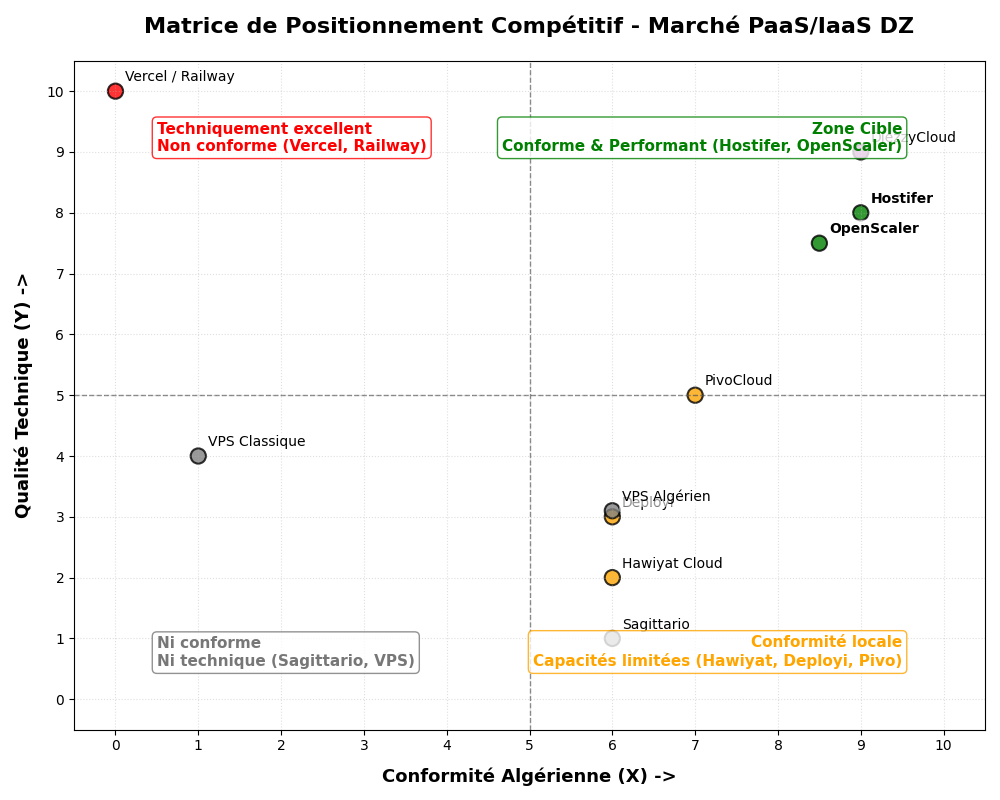
\includegraphics[width=1\linewidth]{5-Chapters/Chapter1/figures/competitive_positioning_matrix_dz.png}
	\caption{Matrice de positionnement compétitif (axes : qualité technique / conformité algérienne)}
	\label{fig:1.5}
	\label{fig:matrice-positionnement}
\end{figure}